\documentclass[10 pt,usenames,dvipsnames, oneside]{article}
\usepackage{../../../modelo-ensino-medio}



\begin{document}

\begin{center}
  \begin{minipage}[l]{3cm}

\includegraphics[width=2cm]{logo}    
\end{minipage}\hfill
\begin{minipage}[r]{.8\textwidth}
 {\Large \scshape Atividade: O problema dos aniversários}  
\end{minipage}
\end{center}
\vspace{.2cm}

\ifdefined\prof
%Habilidades da BNCC
\begin{objetivos}
\item a
\end{objetivos}

%Caixa do Para o Professor
\begin{goals}
%Objetivos específicos
\begin{enumerate}
\item Calcular a probabilidade de um evento usando a propriedade do evento complementar.
\end{enumerate}

\tcblower

%Orientações e sugestões
Para resolver esse problema será necessário fazer algumas suposições: 
\begin{itemize}
\item considerar apenas anos não bissextos; 
\item supor que os $365$ dias do ano são igualmente prováveis como datas de aniversário. Com essas suposições, será adotada a interpretação clássica de probabilidade para resolver o problema.
\end{itemize}

Faça uma enquete perguntando quem são os nascidos em janeiro, fevereiro, etc., até obter uma coincidência (ou não) de aniversários. Se a sua turma tem $35$ ou mais alunos, é muito mais provável que exista uma coincidência de aniversários do que não exista. A explicação para isso envolve o fato de que com $35$ pessoas pode-se formar $595$ pares de datas de aniversário de duas pessoas diferentes, ao passo que no ano há $365$ dias como possíveis datas de aniversário. Para calcular a probabilidade também será necessária pelo menos uma calculadora científica básica.

É importante destacar que a escolha do número $35$ alunos deveu-se à restrição numérica nas calculadoras científicas básicas. Para números maiores do que $35$, as calculadoras apontam “Erro matemático”{} por conta da magnitude de valores manipulados no cálculo da probabilidade, que superam a capacidade de uma calculadora simples. No entanto, usando programação tais probabilidades podem ser facilmente obtidas para números maiores do que $4$. No link há uma ilustração sobre o comportamento dessa probabilidade em função do tamanho do grupo.
\end{goals}

\bigskip
\begin{center}
{\large \scshape Atividade}
\end{center}
\fi

Numa turma de seu colégio há $35$ alunos. Calcule a probabilidade de que haja pelo menos uma coincidência de datas de aniversário (dia e mês) entre os alunos dessa turma. Considere apenas anos não bissextos e suponha que todos os $365$ dias do ano são igualmente prováveis como datas de aniversário.

\begin{figure}[H]
\centering

\noindent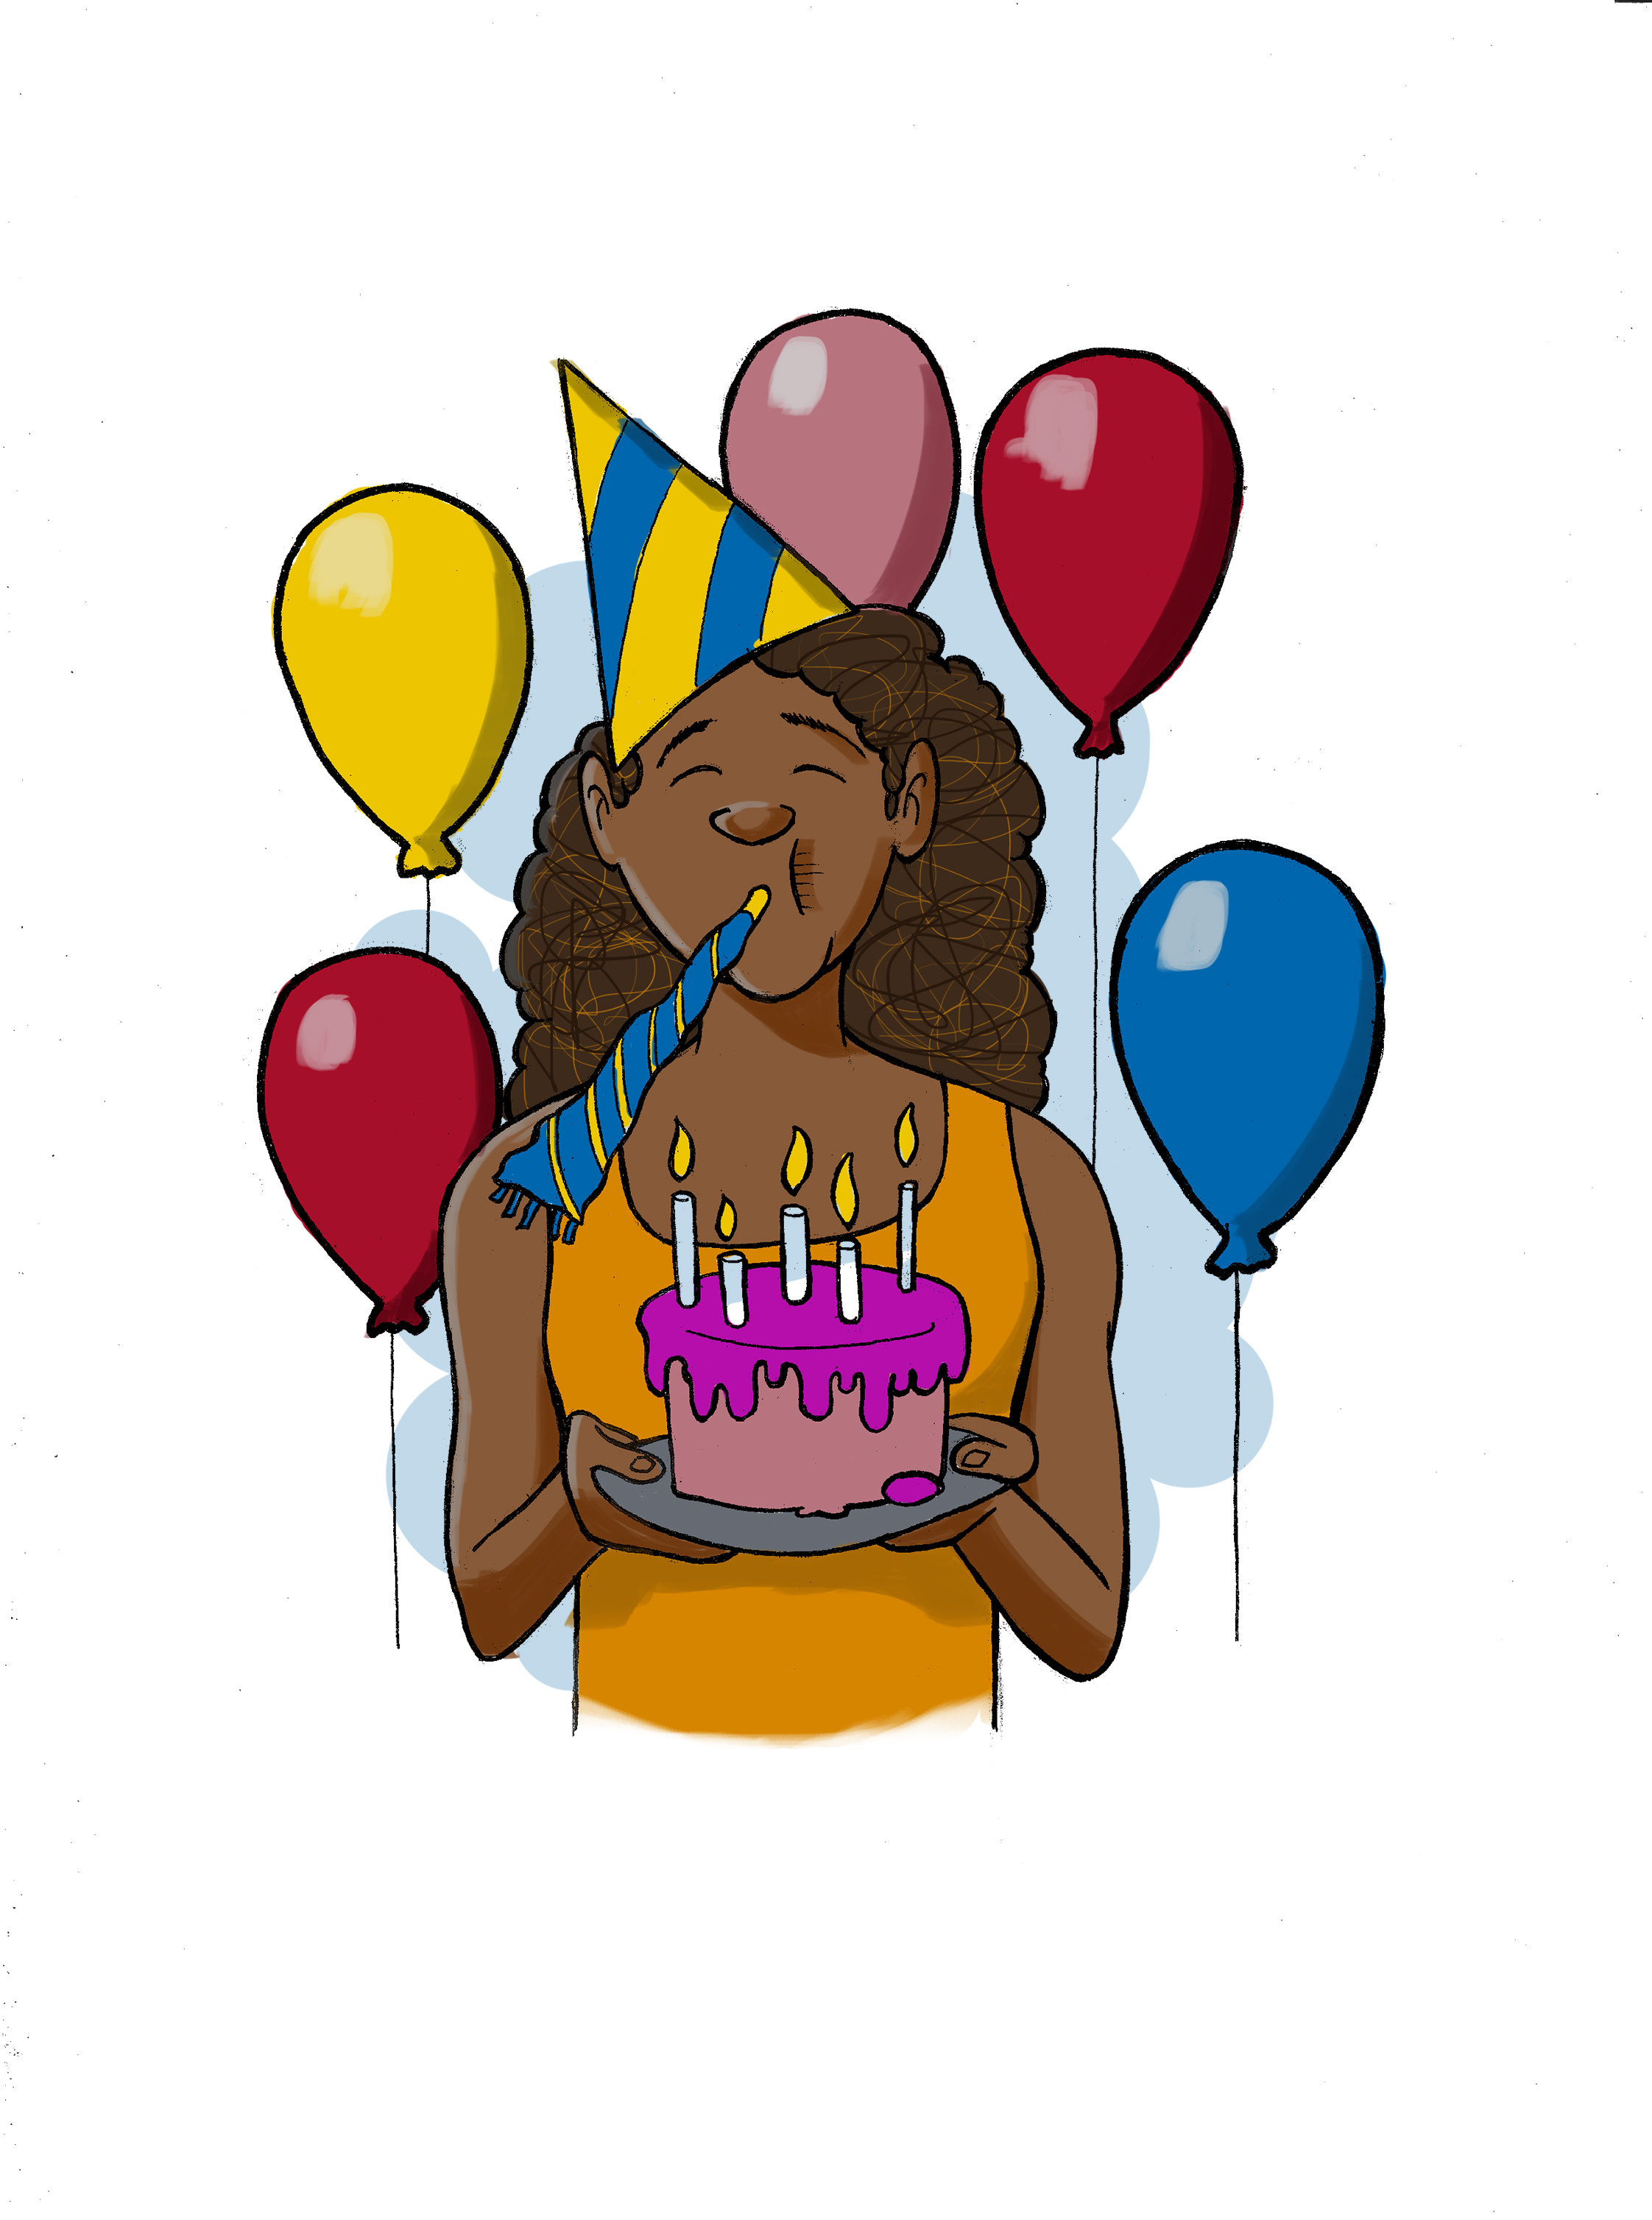
\includegraphics[width=200bp]{bolo.jpg}
\end{figure}

\ifdefined\prof
\begin{solucao}

Calcular diretamente essa probabilidade é muito complicado, pois existem várias configurações possíveis de coincidências de aniversários. Por outro lado, podemos pensar no evento complementar ao evento cuja probabilidade queremos calcular. O evento complementar corresponde ao evento “todos os alunos da turma nasceram em dias diferentes”. Vamos usar a interpretação clássica de probabilidade supondo que todas as configurações possíveis de aniversário para as 40 pessoas são igualmente prováveis e, assim, 
\begin{equation*}
P(\overline{A})=\frac{\#(\overline{A})}{\#(S)}
\end{equation*}. 

Observe que para cada pessoa existem $365$ possibilidades de datas. Como são 35 pessoas, tem-se $\#(S)=365^35$. Agora o número de elementos do evento $\overline{A}$, que corresponde a todos terem nascido em dias diferentes, pode ser calculado, usando o princípio multiplicativo, da seguinte forma: há $365$ possibilidades para o aluno número $1$ da chamada, logo há $(365-1)=364$ possibilidades para o aluno número $2$ da chamada. Continuando, há $(365-2)=363$ possibilidades para o aluno número $3$ da chamada, até $(365-34)=331$ possibilidades para o aluno de número 35 da chamada. Assim, 
\begin{equation*}
\#(\overline{A})=365\cdot364\cdot363\cdots331=\frac{365!}{(365-34)!}.
\end{equation*}

Com uma calculadora científica básica, é possível obter o valor de 
\begin{equation*}
P(\overline{A})=\frac{365!}{(365−35)!}{365^35}
\end{equation*}
que é, aproximadamente, $0{,}814$. A título de informação veja na tabela a seguir as probabilidades de coincidência em função do tamanho do grupo $k$.

\begin{table}[H]
\centering

\setlength\tabcolsep{7.5pt}
\begin{tabular}{|f|f|}
\hline
\tmat{k} & \tmat{P(A)} \\
\hline
5 & 0{,}027 \\
\hline
10 & 0{,}117 \\
\hline
20 & 0{,}411 \\
\hline
22 & 0{,}476 \\
\hline
23 & 0{,}507 \\
\hline
30 & 0{,}569 \\
\hline
40 & 0{,}891 \\
\hline
50 & 0{,}970 \\
\hline
60 & 0{,}994 \\
\hline
\end{tabular}
\end{table}

\end{solucao}
\fi

\end{document}